\documentclass[11pt,a4paper]{article}
\usepackage[utf8]{inputenc}
\usepackage[T1]{fontenc}
\usepackage{lmodern}
\usepackage[margin=1.8cm]{geometry}
\usepackage{graphicx}
\usepackage{hyperref}
\usepackage{enumitem}
\usepackage{titlesec}
\usepackage{multicol}

\setlist{nosep,leftmargin=1.2em}
\titlespacing*{\section}{0pt}{0.6em}{0.3em}
\titleformat{\section}{\normalfont\bfseries\large}{\thesection}{0.5em}{}
\titleformat{\subsection}{\normalfont\bfseries}{\thesubsection}{0.5em}{}
\setlength{\parskip}{0.2em}
\setlength{\parindent}{0pt}

\title{\vspace{-1.5cm}Rapport final --- Simulateur SHDL (\textsc{ArchiDu7})}
\author{Projet Long SHDL\\[0.4em]
\normalsize Contenu rédigé par Arthur Madar \quad{}---\quad{} Diagrammes de classes réalisés par Alexis Briend}
\date{23 mai 2026}

\begin{document}
\maketitle
\vspace{-2em}

\section*{Rappel du sujet}
Créer une application capable de simuler des circuits logiques à partir de scripts SHDL.

\section*{Features}
\begin{itemize}
  \item \textbf{Interprétation du langage et modélisation}~: pouvoir transformer un script SHDL en une modélisation de circuit logique. Cette feature est complétée, elle avait été principalement faite au sprint~1 et~2 mais il restait des choses à ajouter pour le sprint~3 (appel de sous module principalement).
  \item \textbf{Simulation}~: pouvoir simuler un circuit logique avec une interface graphique dédiée. Cette feature est complétée, elle avait été principalement faite au sprint~1 et~2 mais il restait des choses à ajouter pour le sprint~3.
  \item \textbf{Éditeur de Texte}~: un éditeur de texte adapté au langage SHDL (coloration syntaxique/autocompletion). Il lui manque une partie de l'autocompletion que nous n'avons pas pu livrer à temps. Cette feature à été implémenté majoritairement durant le sprint~2 mais quelques ajouts et corrections ont pu être effectués au sprint~3.
  \item \textbf{Interface graphique}~: l'interface graphique de l'application. Celle-çi à été principalement faite au sprint~3, les sprints précédent ne fournissait qu'un squelette.
  \item \textbf{Script de test}~: pouvoir lancer des script de test simple sur une simulation. Seul l'essentiel a pu être terminé, d'autres fonctionnalités prévues n'ont pas pu être implémentées. Cette features à été démarré durant le sprint~3.
\end{itemize}

\section*{Paquettages}
\begin{multicols}{3}
\begin{itemize}
  \item editeur
  \item editeur.autocompletion
  \item editeur.colorisation
  \item boutons
  \item erwan
  \item sauvegarde
  \item parser
  \item parser.automate
  \item parser.conversion
  \item parser.lexer
  \item parser.regex
  \item parser.ll1
  \item parser.ll1.grammar
  \item parser.ll1.tabledriven
  \item parser.ll1.tabledriven.cst
  \item parser.ll1.tabledriven.table
  \item util
  \item simulateur
  \item simulateur.affichage
  \item simulateur.appel
  \item simulateur.scriptTest
\end{itemize}
\end{multicols}

\section*{Diagramme de classe}

\subsection*{Le parser}
\begin{center}
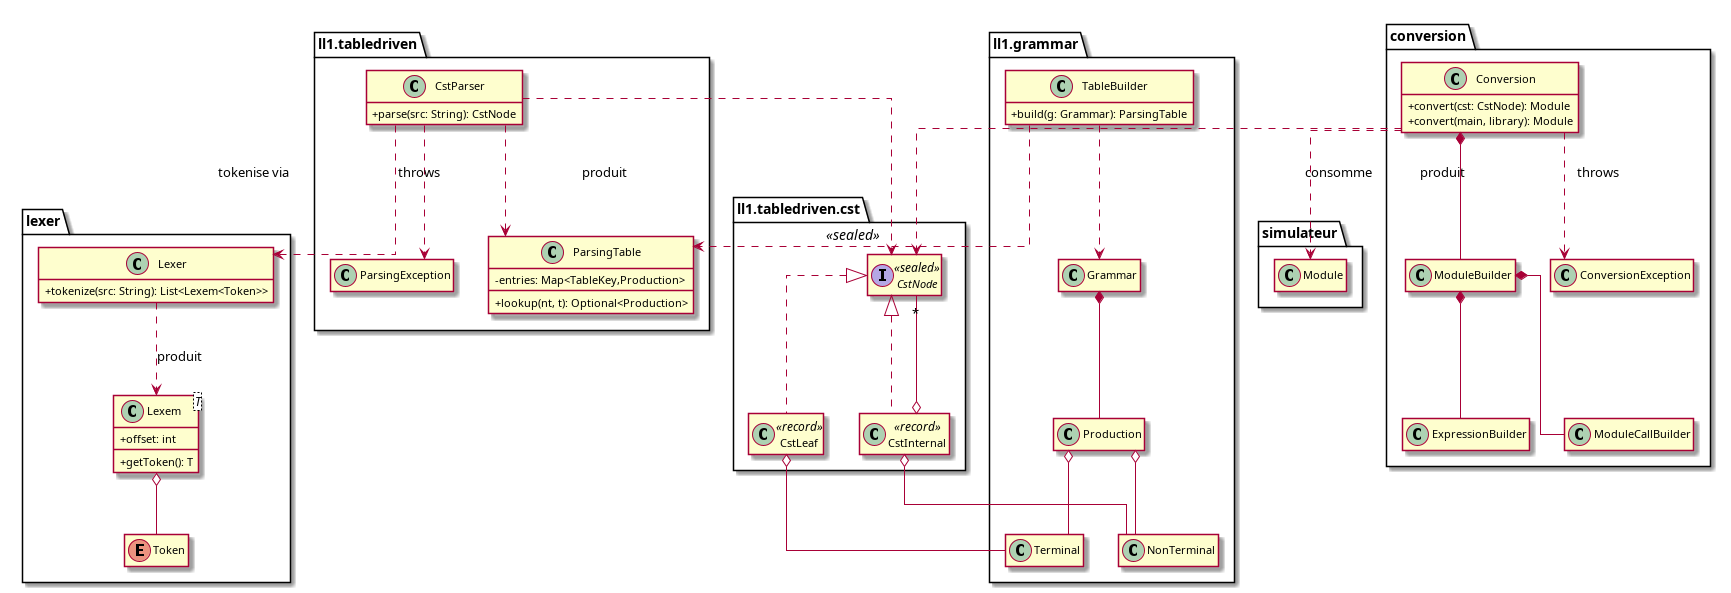
\includegraphics[width=\textwidth]{../parser-classes.png}
\end{center}

\subsection*{La simulation}
\begin{center}
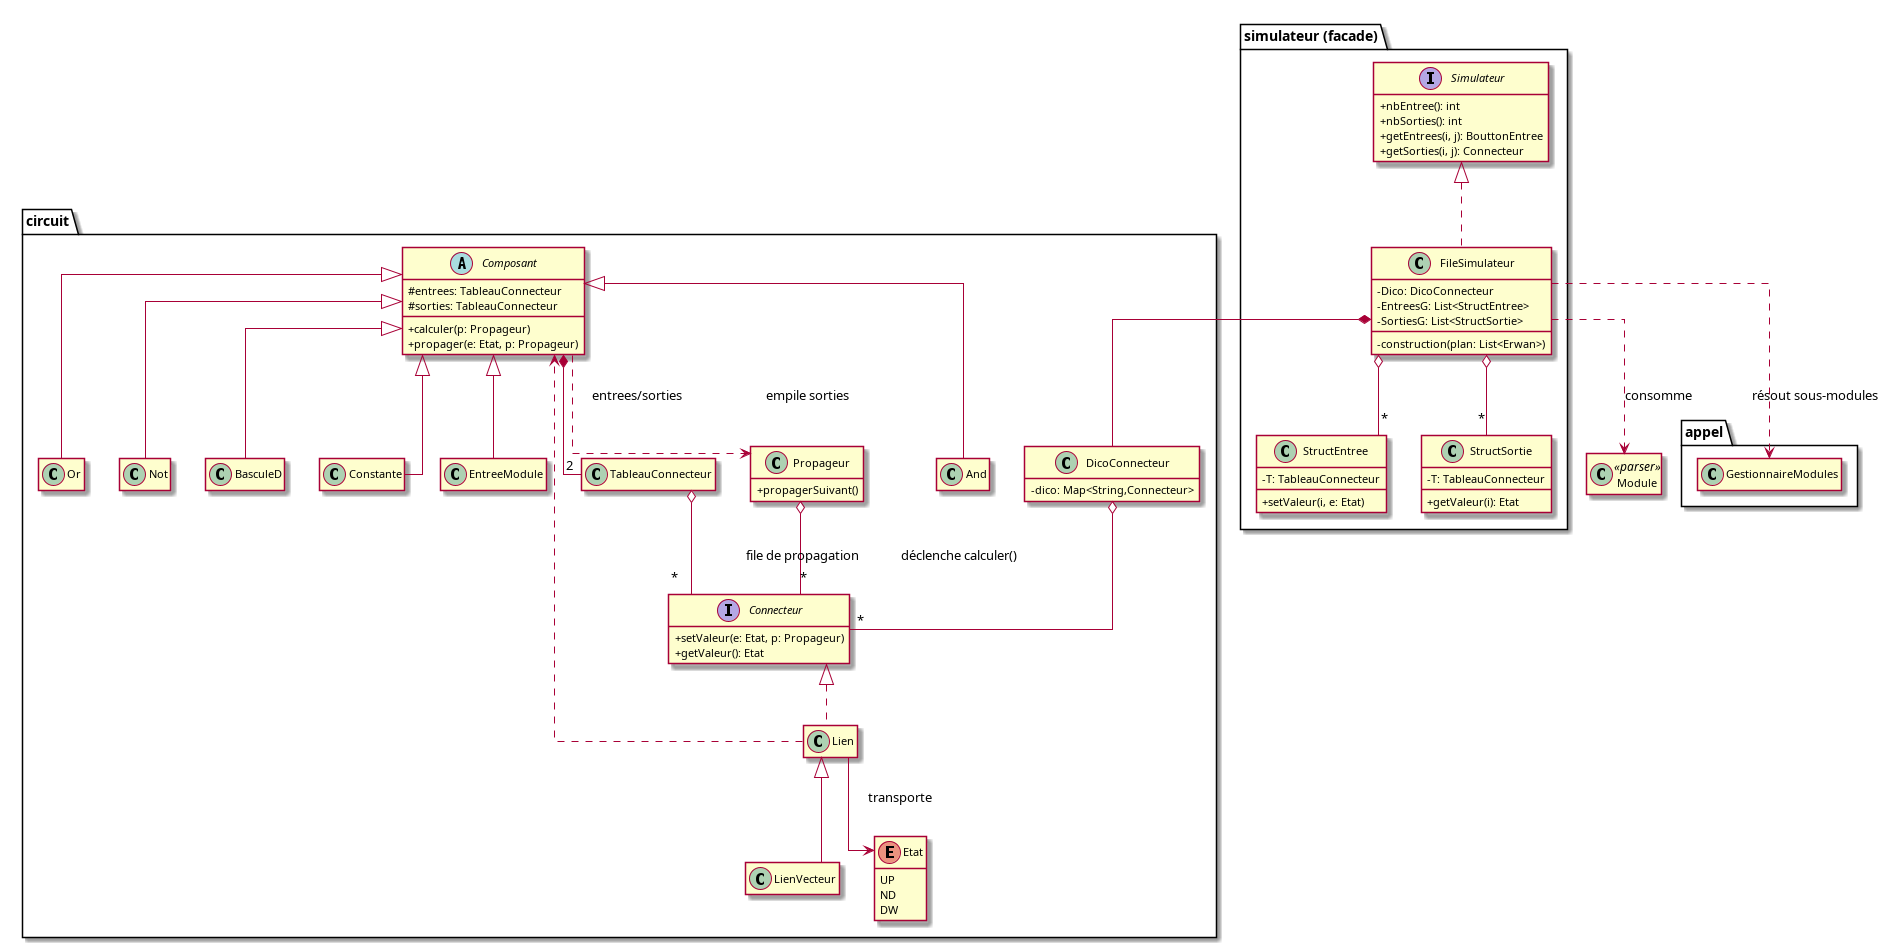
\includegraphics[width=\textwidth]{../simulation-classes.png}
\end{center}

\subsection*{L'éditeur de texte}
\begin{center}
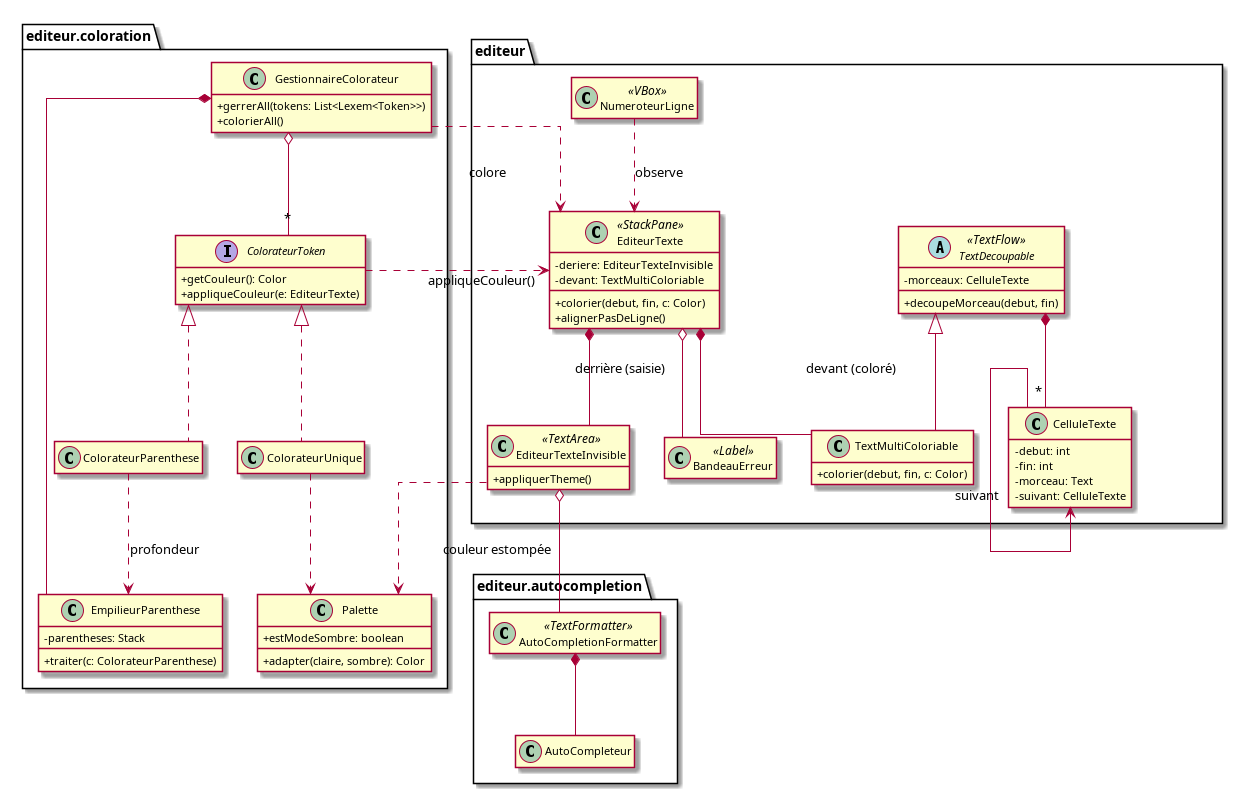
\includegraphics[width=\textwidth]{../editeur-classes.png}
\end{center}

\subsection*{Architecture globale de l'interface}
\begin{center}
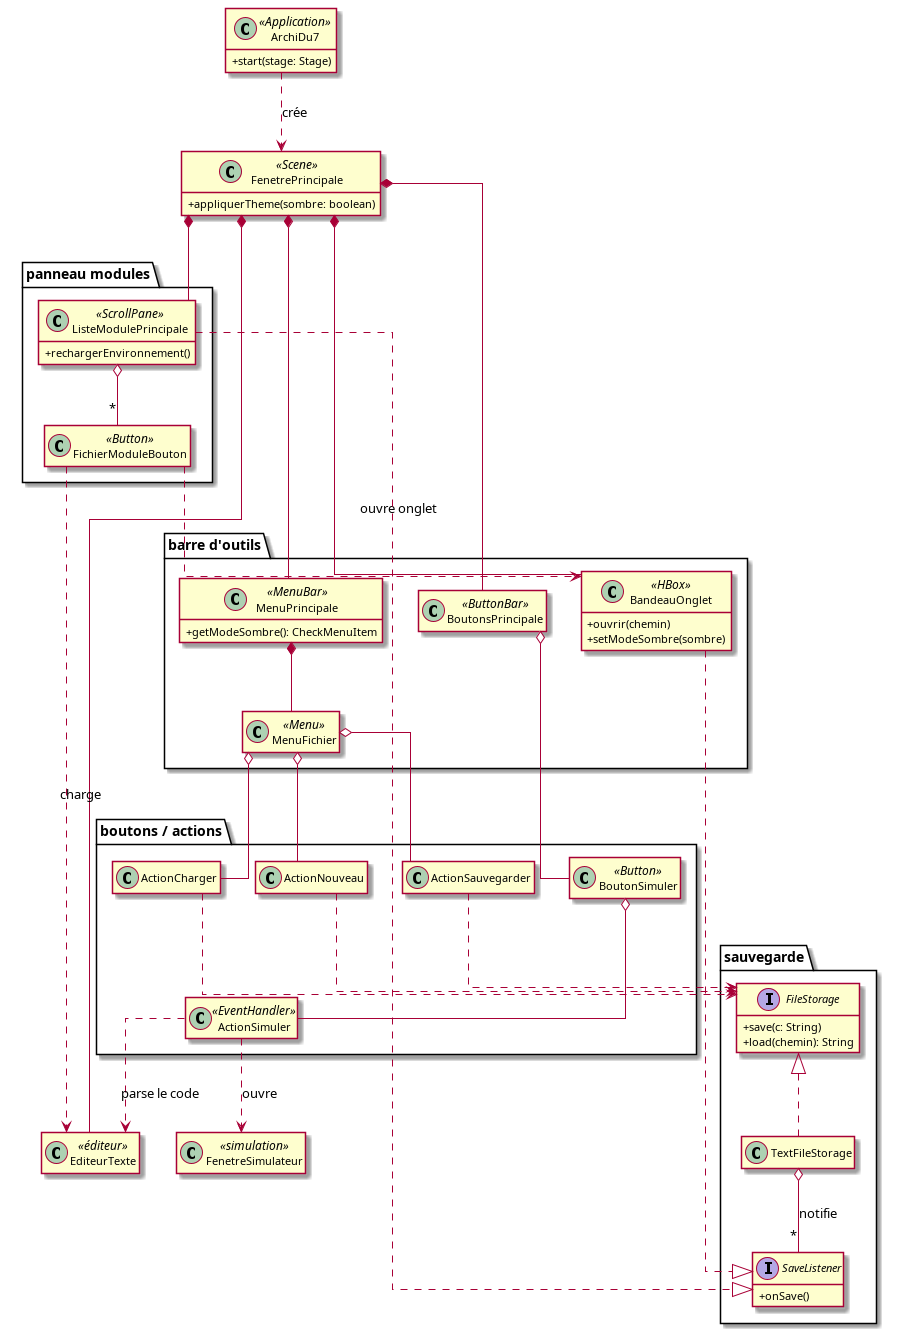
\includegraphics[height=0.9\textheight]{../interface-classes.png}
\end{center}

\section*{Dynamique du système}

\section*{Choix de conception}
\begin{itemize}
  \item Utilisation de javafx afin de pouvoir utiliser du css dans le code.
  \item Les simulations apparaissent dans une fenêtre séparée du reste.
  \item Les fichiers SHDL sont scannés d'un même dossier \texttt{modules/}.
  \item La transformation du module en circuit n'est calculée que lorsque l'on veut lancer sa simulation.
\end{itemize}

\section*{Problèmes de conception rencontrés}
\begin{itemize}
  \item Initialement, l'état des potentiel dans le circuit était calculé en mettant à jour tous les potentiels mais cela créait un problème de logique séquentielle donc nous avons mis en place une méthode de calcul par propagation (parcours en largeur).
  \item La classe TextArea en javafx ne permet de colorier des morceaux indépendant de texte. Nous avons donc décidé d'afficher du texte coloriable par morceau (de notre propre implémentation) par dessus le TextArea pour donner l'illusion d'une coloration syntaxique.
\end{itemize}

\section*{Organisation de l'équipe}
\begin{itemize}
  \item Nous avons découpé l'effectif entre la partie interface graphique/éditeur de texte et la partie modélisation/simulation.
  \item Nous nous répartissions les tâches à l'aide de Jira.
  \item À partir du sprint~2, nous faisions un appel vocal tous les mercredis pour faire un point sur l'avancement du projet.
  \item Nous avons fait un groupe de discussion discord pour nous partager les avancées de chaque parties et nous poser des questions.
\end{itemize}

\end{document}
